\section{Δεδομένα Ελέγχου - Προ επεξεργασία}
\label{Dataset, Preprocessing}

\subsection{Σύνολο Δεδομένων DTU, \enit{DTU Robot Image Datasets} \cite{aanaes2016large}}
Το σύνολο δεδομένων DTU MVS 2014 \cite{aanaes2016large}, αποτελεί μια συλλογή εικόνων τρισδιάστατων μοντέλων πολλαπλών όψεων. Το συγκεκριμένο σύνολο δεδομένων περιέχει 80 σκηνές μεγάλης φωτομετρικής ποικιλίας, δηλαδή 80 διαφορετικά μοντέλα που φωτογραφήθηκαν με χρήση ρομποτικού βραχίονα κάτω από ίδιες συνθήκες φωτισμού και τοποθέτησης της κάμερας. Συγκεκριμένα κάθε σκηνή περιέχει είτε 49 είτε 64 διαφορετικές ακριβείς θέσεις καμερών και σαρώσεις δομημένου φωτός, όλες αποκτημένες από ρομποτικό βραχίονα 6 βαθμών ελευθερίας (6-DOF).

\begin{figure}
    \centering
    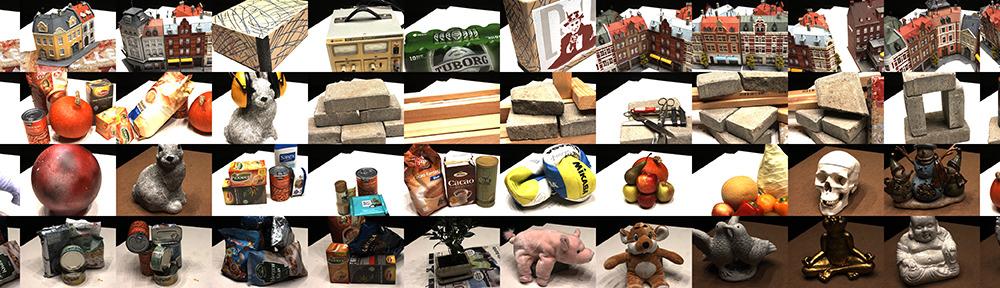
\includegraphics[width=\linewidth]{images/chapter4_img/dtu.jpg}
    \caption{DTU MVS σύνολο δεδομένων}
    \label{fig:dtu}
\end{figure}

\subsection{Εξαγωγή Δεδομένων Τρισδιάστατης Στερεομετρίας σε ένα αντικείμενο Scene Dataset}
Για να γίνει εκπαίδευση του δικτύου και να γίνει επίβλεψη του με το σύνολο δεδομένων εικόνων που έχει το DTU γίνεται χρήση μια κλάσης που αποτελεί την δομή δεδομένων που αποθηκεύει σύνολο εικόνων μια σκηνής. Συγκεκριμένα η κλάση \enit{SceneDataset} δέχεται τις εικόνες μια σκηνής (που την δεδομένη στιγμή αναπαριστά το δίκτυο απόδοσης), τις μάσκες των ενδιαφέρον ή ενεργών pixel για τα αντικείμενα της σκηνής. Κάνοντας χρήση του ευρετηρίου της κάμερας σε συνδυασμό έναν πίνακα κλίμακας \enit{scale matrix} μαζί με τις παραμέτρους των καμερών (βλ. Κεφ.\ref{appendix:camerasystem}) που στοχεύουν το αντικείμενο δημιουργεί το αντικείμενο της κάμερας όπως περιγράφεται στο παράρτημα. Σε περίπτωση που δεν υπάρχουν δεδομένες θέσεις καμερών,  χρειάζεται να οριστούν οι αρχικές θέσεις των καμερών με μια αιτιοκρατική μέθοδο που υπάγεται στην προ επεξεργασία καμερών. Συγκεκριμένα γίνεται χρήση της μεθόδου \cite{jiang2013global}, που είναι σε θέση να κάνει μια καθολική γραμμική αρχικοποίηση αυτών των παραμέτρων αν δεν παρέχονται από το σύνολο δεδομένων. Στην συνέχεια αυτές οι παράμετροι εκπαιδεύονται μιας και αναπαριστούν κάμερες με θόρυβο(για περισσότερα βλ. Κεφ.\ref{appendix:camerainitrepresent}). Έτσι το αντικείμενο σε κάποιο δείκτη μπορεί να δώσει κανονικοποιημένες εγγενείς παραμέτρους κάμερας, pixel των πολλαπλών εικόνων της σκηνής που εκτιμάται κατά την φωτογράφιση καθώς και της αντίστοιχη μάσκα. Ταυτόχρονα σε περίπτωση εκπαιδεύσιμων παραμέτρων κάμερας δίνει και την πόζα \footnote{quaternion πίνακας με το πίνακα στροφής της κάμερας} της κάμερας που εκτιμάται ότι έχει. Παράλληλα το αντικείμενο επιστρέφει και τα pixel της πραγματικής εικόνας, δηλαδή όχι την φωτογραφία της παρούσας σκηνής που αναπαριστά το έμμεσο πεδίο. 

Παράλληλα παρέχεται συνάρτηση που συνενώνει όλα αυτά τα δεδομένα σε τανυστές και η συνάρτηση που εκτιμά την αρχική πόζα της κάμερας.  